\documentclass[11pt]{report}
\usepackage[utf8]{inputenc}
\usepackage[margin=1in]{geometry}
\usepackage{amsfonts,amsmath,amssymb}
\usepackage[none]{hyphenat}
\usepackage[utf8]{inputenc}
\usepackage{fancyhdr}
\usepackage{graphicx}
\graphicspath{{images/}}
\usepackage[nottoc, notlot, notlof]{tocbibind}
\usepackage[spanish]{babel}
\usepackage{enumitem}
\usepackage{hyperref}
\usepackage{eurosym}
\usepackage[T1]{fontenc}
\usepackage{mathpazo} 
\usepackage{listings}
\usepackage{xcolor}
\usepackage{textcomp}
\usepackage{eurosym}
\usepackage{amsmath}
\usepackage{amssymb}
\usepackage{textcomp}
\usepackage{gensymb}
\usepackage{appendix}
\setlength\parindent{24pt}
\renewcommand{\lstlistingname}{Extracto de código}
\renewcommand{\lstlistlistingname}{Conjunto de código}

\renewcommand{\UrlFont}{\ttfamily\small}

\pagestyle {fancy}
\fancyhead{}
\fancyfoot{}
\fancyhead[L]{\slshape\MakeUppercase{Trabajo de fin de grado}}
\fancyhead[R]{\slshape Ionut Morariu}
\fancyfoot[C]{\thepage}


\parindent 0ex
%\setlength{\parindent}{4em} %Change indent width
%\setlength{\parskip}{1em} %space between paragraphs

\lstdefinelanguage{JavaScript}{
  morekeywords=[1]{break, continue, delete, else, for, function, if, in,
    new, return, this, typeof, var, void, while, with},
  % Literals, primitive types, and reference types.
  morekeywords=[2]{false, null, true, boolean, number, undefined,
    Array, Boolean, Date, Math, Number, String, Object},
  % Built-ins.
  morekeywords=[3]{eval, parseInt, parseFloat, escape, unescape,console},
  sensitive,
  morecomment=[s]{/*}{*/},
  morecomment=[l]//,
  morecomment=[s]{/**}{*/}, % JavaDoc style comments
  morestring=[b]',
  morestring=[b]"
}[keywords, comments, strings]

\lstalias[]{ES6}[ECMAScript2015]{JavaScript}

\lstdefinelanguage[ECMAScript2015]{JavaScript}[]{JavaScript}{
  morekeywords=[1]{await, async, case, catch, class, const, default, do,
    enum, export, extends, finally, from, implements, import, instanceof,
    let, static, super, switch, throw, try},
  morestring=[b]` % Interpolation strings.
}

% Requires package: color.
\definecolor{mediumgray}{rgb}{0.3, 0.4, 0.4}
\definecolor{mediumblue}{rgb}{0.16, 0.5, 0.73}
\definecolor{forestgreen}{rgb}{0.13, 0.55, 0.13}
\definecolor{darkviolet}{rgb}{0.58, 0.0, 0.83}
\definecolor{royalblue}{rgb}{0.25, 0.41, 0.88}
\definecolor{crimson}{rgb}{0.86, 0.8, 0.24}
\definecolor{lightgrey}{rgb}{0.97, 0.97, 0.97}
\definecolor{black}{rgb}{0.05, 0.05, 0.1}
\definecolor{green}{rgb}{0.1529, 0.6823, 0.3764}
\definecolor{red6}{rgb}{0.753, 0.224, 0.169}

\lstdefinestyle{JSES6Base}{
  backgroundcolor=\color{lightgrey},
  basicstyle=\fontsize{7}{9}\selectfont\ttfamily,
  breakatwhitespace=false,
  breaklines=false,
  captionpos=b,
  columns=fullflexible,
  commentstyle=\color{mediumgray}\upshape,
  emph={},
  emphstyle=\color{crimson},
  extendedchars=true,  % requires inputenc
  fontadjust=true,
  frame=single,
  identifierstyle=\color{black},
  keepspaces=true,
  keywordstyle=\color{mediumblue},
  keywordstyle={[2]\color{darkviolet}},
  keywordstyle={[3]\color{red}},
  numbers=left,
  numbersep=10pt,
  numberstyle=\tiny\color{black},
  rulecolor=\color{black},
  showlines=true,
  showspaces=false,
  showstringspaces=false,
  showtabs=false,
  stringstyle=\color{green},
  tabsize=2,
  title=\lstname,
  upquote=true  % requires textcomp
}

\lstdefinestyle{JavaScript}{
  language=JavaScript,
  style=JSES6Base
}
\lstdefinestyle{ES6}{
  language=ES6,
  style=JSES6Base
}

\begin{document}
\begin{titlepage}



\begin{center}
	
\includegraphics[scale=1]{cabecera}\\
	\vspace*{1cm}
	\Large{\textbf{\MakeUppercase{Universidad Politécnica de Madrid}}}\\[3mm]
	\Large{{\MakeUppercase{Escuela técnica de ingeniería y diseño industrial}}}\\[3mm]
	\Large {Grado en Ingeneriería Eléctrica}\\
	\vfill
	\line(1,0){400}\\
	\Large{{\MakeUppercase{Trabajo de fin de grado}}}\\
	\Huge{\textbf{Aplicación web para la estimación del coste de una instalación solar conectada a red}}\\[5mm]
	\Large{Autor: Ionut Cristian Morariu}\\
	\line(1,0){400}\\
	\vfill
\end{center}
\begin{flushright}
\Large {Tutor: Óscar Perpiñán Lamigueiro}\\[3mm]
\Large{Departamento de Ingeniería Eléctrica,\\ Electrónica, Automática y Física aplicada}\\[10mm]
Madrid, \today
\end{flushright}

\end{titlepage}

\renewcommand{\baselinestretch}{1.5} %line spacing
\renewcommand{\labelitemi}{\textbullet}

\tableofcontents
\thispagestyle{empty}
\clearpage

\setcounter{page}{1}


\chapter{Introducción}
\section{Objetivos}
El objetivo de este proyecto es el desarrollo de una aplicación o página web de fácil acceso para todos los usuarios, con la finalidad de ofrecer una estimación inicial del coste y la posible generación de una instalación fotovoltaica doméstica de conexión a red.\\

Durante el resto del documento, si fuera necesario, se hará referencia a la aplicación desarrollada en este proyecto en el nombre de SolarCalc.\\

Para poder llevar a cabo esta estimación, el usuario introducirá unos serie de datos acerca de su emplazamiento y edificación en la que desea situar la instalación, y la aplicación hará todos los cálculos necesarios para ofrecer una aproximación lo más cercana al resultado final teniendo en cuenta todas la variables que puedan intervenir.\\

La aplicación también ofrecerá otros datos de posible interés para el usuario como: el número de paneles que se pueden instalar, la potencia de dichos paneles y la potencia del inversor.\\

La idea de esta aplicación surge de una conversación que tuve con un conocido cuando estaba planificando la construcción de su nueva vivienda, en la cual quería realizar una instalación fotovoltaica para reducir el gasto en la factura de electricidad.\\

En su búsqueda no encontró ningún servicio que fuera lo suficientemente sencillo de entender para una persona sin ningún tipo de conocimiento previo acerca de la generación fotovoltaica, que le aportase la posibilidad de poder personalizar los cálculos a su emplazamiento y planos de construcción.\\

Otro de los puntos clave de la aplicación es que sea de código abierto y gratuita para los usuarios, usando fuentes de información disponibles para cualquier interesado. Todos los pasos y operaciones se podrán obtener, analizar y reutilizar de manera gratuita desde un repositorio de Github \footnote{\textit{Github.com:} Plataforma online de almacenamiento de código y documentación de fuentes abiertas.}.\\


Los objetivos detallados de esta aplicación son los siguientes:
\begin{itemize}
\item Diseñar una interfaz de usuario amigable y sencilla de usar para que la pueda utilizar un gran número de personas sin necesidad de conocimientos sobre energía fotovoltaica.

\item Obtención de los datos de irradiación en el emplazamiento indicado por el usuario mediante el uso de API\footnote{\textit{Application Programming Interface}: conjunto de funciones y procedimientos que ofrece la posibilidad de un software a interaccionar con otro.} externas.
\item Realizar todos los cálculos necesarios para ofrecer una estimación competente de los siguientes datos:

\begin{itemize}

\item Número de paneles que se pueden instalar.
\item Potencia máxima a instalar.
\item Potencia del inversor.
\item Energía eléctrica producida en un año.

\end{itemize}
\end{itemize}

\section{Análisis previo de soluciones}\label{intro_solutions}

Antes de comenzar el desarrollo del proyecto, se llevó a cabo una revisión de las soluciones existentes de estimaciones de instalaciones fotovoltaicas existentes en el mercado para decidir si tenía cabida una aplicación como la que se iba a desarrollar.\\

Algunas de las soluciones encontradas fueron:

\begin{enumerate}
\item \textbf{PVSyst - Photovoltaic Software}

El software PVSyst, desarrollado por la empresa suiza con el mismo nombre es quizá el más conocido dentro del ámbito del estudio y la estimación de instalaciones fotovoltaicas. Ofrece una amplia capacidad de personalización de todos los componentes de la instalación.

\item \textbf{CalculationSolar.com}

Es el primer resultado de Google al buscar el término \textit{``calculadora de instalaciones fotovoltaicas''}, por tanto será una de las primeras aplicaciones que una persona que desea realizar una instalación en su vivienda visite.

\item \textbf{SISIFO}

Es una herramienta web diseñada y desarrollada por el Grupo de Sistemas Fotovoltaicos del Instituto de Energía Solar de la Universidad Politécnica de Madrid. Ha sido y es la herramienta interna utilizada por los ingenieros de dicho grupo.

\item \textbf{PVGIS}

Aplicación web desarrollada por el \textbf{European Commission Joint Research Center} desde 2001. Su enfoque es asistir en el calculo y estimación de instalaciones fotovoltaicas, ya sean conectadas a red, de seguimiento o de autoconsumo.

\item \textbf{System Advisor Model}

System Advisor Model (SAM), desarrollado por el Laboratorio Nacional de Energías Renovables, perteneciente al Departamento de Energía del gobierno americano, es una software técnico-económico gratuito que ayuda a la toma de decisiones en el amplio campo de las energías renovables. Ofrece un conjunto de soluciones muy completas no solamente relacionadas con la energía fotovoltaica, sino también termosolar, eólica, geotermal o biomasa, entre otras.

\item \textbf{solaR}

solaR es un paquete de código para el entorno de R, desarrollado por Oscar Perpiñán, que a pesar de tener objetivos diferentes a los planteados por la aplicación desarrollada en este proyecto, ha servido como base para validar todos los cálculos que se han realizado en ella.
\end{enumerate}

En el apartado \ref{existing_solutions}  se lleva a cabo un desarrollo mas detallado de las características de las soluciones mencionadas así como sus diferencias con la propuesta de este proyecto.

\section{Aspectos técnicos}

Para construir cualquier página web se deben desarrollar dos sistemas diferentes llamados Backend y Frontend.
El Backend es el la parte de cálculo y tratamiento de peticiones, comúnmente llamado server o servidor. Por otro lado se encuentra el Frontend que es la parte de cara al usuario, la que se encarga de recoger los datos introducidos por este y enviarlos al servidor.

\subsection{Backend}

Para el Backend se ha empleado una tecnología basada en Javascript llamada NodeJS \footnote{\textit{NodeJS:} Entorno de ejecución basado en el motor de Chrome llamado V8. \url{https://nodejs.org/en/} }, con la ayuda de las librerias ExpressJS\footnote{\textit{ExpressJS:} Framework web para el entorno de NodeJS. \url{https://expressjs.com/es/}} y Mongoose \footnote{\textit{Mongoose:} Capa intermedia de interacción para las BBDD MongoDB \url{https://mongoosejs.com/}}.   \\
La base de datos que se ha utilizado para almacenar los datos necesarios ha sido MongoDB.

En el servidor se realizan varias tareas relacionadas con los cálculos necesarios. Algunas de estas tareas son:
\begin{itemize}
\item Obtención de los datos de irradiación global media en el plano horizontal para el emplazamiento indicado
\item Proceso completo de cálculo para pasar de la irradiación en el plano horizontal al plano inclinado y orientado según los datos introducidos por el usuario
\item Proceso de obtención de los datos relacionados con el perfil horario de temperatura en el emplazamiento indicado
\item Gestión de las diferentes rutas que constituyen la API.
\end{itemize}

\subsection{Frontend}
 Para el Frontend de la página se han utilizado las tres tecnologías necesarias para poder desarrollar una pagina web: HTML5, CSS3, Javascript.\\
 

Esta parte de la página es la encargada de recoger los datos del usuario  y enviarlos al servidor para que se realicen los cálculos. Una vez realizados dichos cálculos, la página mostrará la información relevante al usuario, junto con algunos unos gráficos adicionales.\\

Tanto el backend como el frontend están almacenados en un servidor de Linux remoto activo 24/7.\\

Todas las tareas mencionadas tanto en la parte de Backend como en la parte de Frontend se describirán en detalle en la sección \ref{sec:theory}, junto con todos los cálculos en los que se ha basado. 

\newpage

\chapter{Estado del arte}

\section{Situación actual de la generación fotovoltaica}
Según el informe anual de la UNEF\footnote{\textit{UNEF}: Unión Española fotovoltaica} en 2019\cite{unef_2019} la evolución de las energías renovables superó incluso las expectativas mas optimistas alcanzando valores próximos a los 100 GW.

Los aspectos que más han influido en estas cifras han sido, entre otros, la reducción drástica del coste de producción de dichas tecnologías. De hecho, la energía fotovoltaica es ya más barata que la generada por plantas de combustibles fósiles en términos de LCOE\footnote{\textit{LCOE}: Levelized Cost of energy: Medición del coste medio de generación de energía de una planta a lo largo de su vida útil }. Según menciona Bloomber Energy Finance, la fotovoltaica seguirá reduciendo sus costes un 34\% hasta 2030.\\

Sumado a la reducción del coste, el aumento de compraventa de energía a largo plazo - que sigue en alza desde 2018, alcanzando los 14 GW - es otro de los factores influyentes en el crecimiento del sector. Así lo es también la reducción del precio de la energía en las subastas, alcanzando valores tan bajos como 20\$/MWh.\\

Concretamente en Europa, el crecimiento anual de la capacidad solar instalada ha sido de un 23\%, con Alemania como líder sumando otros 2,95 GW respecto a la capacidad del año anterior. En segundo y tercer lugar se encuentran Turquía y los Países Bajos.\\

Bajando un nivel más, nos encontramos con el mercado español, que, según estimaciones del mismo informe de la UNEF, la potencia total instalada experimentó un crecimiento significativo, llegando hasta el valor de 262 MW, sumando la potencia instalada tanto de generación centralizada como la de autoconsumo.\\

Para este año 2020 se estima se estima que la instalación de energía fotovoltaica alcance el umbral de los 20 GW. Si se cumplen las expectativas, la capacidad podría llegar a alcanzar los 200 GW para 2023.\\

Un papel importante lo juegan las autoridades tanto nacionales como a nivel europeo, que apuestan por las fuentes de energías limpias. Para ser exactos, el año 2018 fue uno de los más relevantes en materia de política energética europea desde que se aprobó el tercer paquete de energía en 2009.

De las ocho propuestas que se aprobaron, destaca por su importancia para el sector fotovoltaico la directiva 2018/2001, en la que se recoge el derecho básico al autoconsumo, individual o colectivo, al almacenamiento y sobretodo a la venta de excedentes.\\

En el panorama español, tras varios años de parálisis debida a la compleja situación política de los últimos años, la energía fotovoltaica volvió a recuperar algo de impulso a final del año 2019. Durante el año 2018 y especialmente el 2019, se han incrementado sustancialmente las instalaciones de fotovoltaica, en gran parte gracias a las expectativas generadas por la eliminación del denominado impuesto al sol y la progresiva suspensión de trabas administrativas todas ellas propiciadas por el nuevo marco legal establecido por la administración pública mediante los Reales Decretos 15/2019 y 244/2019.

Según datos proporcionados por la Red Eléctrica Española \footnote{\url{https://www.ree.es/es/datos/publicaciones/series-estadísticas-nacionales}}, la potencia instalada en España ha experimentado un crecimiento de 1,2GW en los últimos 4 años, pasando de 4.6 GW en 2016 a 5.8 GW en 2019.

Se trata del mayor ritmo de crecimiento desde 2008, cuando se instalaron cerca de 2.7 GW de nueva potencia. Es una buena noticia, pero no exenta dificultades debidas sobre todo a la unidireccionalidad de la red eléctrica de nuestro territorio. Sin ir mas lejos, el operador técnico del sistema, REE ha denegado la instalación de 26,3 GW de nueva potencia debido a la imposibilidad de los nudos para gestionar la energía producida por dicha capacidad.

Esto no significa que dicha energía no se vaya a instalar, sino que habrá que esperar a la nueva planificación energética prevista para el periodo 2021-2026 en la que ya están trabajando tanto la REE como las comunidades autónomas para brindar mas oportunidades para los sistemas de conexión a red.\\

En definitiva, como podemos observar, las energías renovables, y en especial la fotovoltaica esta dando mucho que hablar y cada vez es una tema más tratado por el público general y por tanto, es un aspecto a tener en cuenta a la hora de construir nuevas edificaciones o mejorar la eficiencia energética de las existentes.

Surge por tanto la necesidad de aplicaciones y soluciones para la estimación de instalaciones fotovoltaicas que sean intuitivas y fáciles de usar para aprovechar el gran interés que está mostrando el público general.

\section{Soluciones existentes y sus carencias} \label{existing_solutions}

Como ya se ha mencionado en el el apartado \ref{intro_solutions}  existen multitud soluciones para la estimación o simulación de instalaciones fotovoltaicas. Sin embargo, es posible que la aplicación descrita en este proyecto siga teniendo cabida porque ofrece ciertas funciones que, en cierta medida, no existen en las soluciones que se han estudiado.

A continuación se describirán con detalle las soluciones mencionadas anteriormente, junto con sus capacidades y carencias.
\pagebreak

\begin{enumerate}
\item \textbf{PVSyst - Photovoltaic Software} \cite{sota_pvsyst}

El software PVSyst, desarrollado por la empresa suiza con el mismo nombre es quizá el más conocido dentro del ámbito del estudio y la estimación de instalaciones fotovoltaicas. Ofrece una amplia capacidad de personalización de todos los componentes de la instalación.

PVSyst es capaz de calcular con amplio detalle el diseño y dimensionado del sistema, zonas de sombra, envejecimiento del material, almacenamiento de energía, entre otras opciones.\\

PVSyst se diferencia de la aplicación que se desarrolla en este proyecto en algunos puntos importantes como:
	\begin{itemize}
		\item Es de pago, con una licencia anual de aproximadamente \euro{568}.
		\item Es un programa que se debe instalar en un ordenador de Windows (No funciona en Linux u OSX).
		\item Es poco intuitivo para un usuario con bajos conocimientos de instalaciones fotovoltaicas.
	\end{itemize}
En resumen, PVSyst es un software mucho mas completo y complejo que la solución que la desarrollada en este proyecto, y que va enfocada a un público con una base sólida sobre energía fotovoltaica.

\item \textbf{CalculationSolar.com} \cite{sota_calculationsolar}

Como ya se ha mencionado en la introducción, CalculationSolar.com es el primer resultado que aparece en el motor de búsqueda de Google cuando se introduce el término \textit{``calculadora de instalaciones fotovoltaicas''} y por tanto será una de las primeras opciones que un usuario que está interesado en realizar una instalación fotovoltaica considere.

A diferencia de PVSyst, CalculationSolar.com es una solución en la web y gratuita, por lo que la barrera de acceso es mas baja.
Nada mas entrar a la pagina lo primero con lo que nos encontramos es con un formulario sencillo sobre el emplazamiento y la configuración de la instalación. La información que se solicita es sencilla e intuitiva, incluso se ofrece la posibilidad de hacer clic en un mapa interactivo para determinar las coordenadas.

Lo siguiente es introducir la información acerca de las necesidades de potencia, dado que esta calculadora esta enfocada a las instalaciones de autoconsumo sin conexión a red.

Una vez introducidos estos datos, el programa realiza los cálculos y nos ofrece un resultado bastante detallado del campo fotovoltaico, el regulador de carga, la batería y el inversor que mejor encajaría con nuestro requisitos.

La principal diferencia con la aplicación que se desarrolla en este proyecto es requisitos versus limitaciones. Es decir, CalculationSolar.com te permite seleccionar tus requisitos de potencia y te indica el generador que vas a necesita para poder hacer frente a dicha carga. En cambio, SolarCalc indica la potencia y energía que se puede llegar a generar con las limitaciones arquitectónicas impuestas por el usuario. 

\item \textbf{SISIFO} \cite{sota_sisifo}

La solución propuesta por el Grupo de Energías Fotovoltaicas del Instituto de Energía Solar de la Universidad Politécnica de Madrid es también un solución web para el calculo de instalaciones solares tanto de bombeo de agua como conectadas a red.

El sistema de input de información del usuario es muy completo. Paso por paso le permite a éste introducir desde los datos geográficos y meteorológicos hasta hasta los valores de perdidas en los diferentes cableados del sistema. No obstante, los valores por defecto son muy válidos así que incluso un usuario con poco conocimiento sobre energía podría llegar a obtener unos resultados fiables.

Una vez realizada la simulación, la aplicación aporta multitud de resultados detallados tales como Irradiaciones en el plano horizontal e inclinado, temperaturas y energía producida.

Esta aplicación es la más parecida, salvando las distancias, a la que se desarrolla en este proyecto. Sin embargo, es posible que puede llegar a abrumar en cierta medida a un usuario que desea solamente conocer cual es la potencia o energía que puede llegar a producir en su casa, para saber si le va a resultar rentable la inversión.

\item \textbf{PVGIS} \cite{sota_pvgis}

PVGIS es la solución desarrollada por el JRC (Centro de Investigación Conjunta), que forma parte del EU Science Hub. Consiste en una aplicación web que nos permite estimar la energía que puede llegar a producir una instalación fotovoltaica en función de los parámetros introducidos por el usuario.

Tras elegir la localización como primer paso, el programa nos abre la posibilidad de elegir el tipo de instalación, entre conectada a red, con seguimiento, o autónomo.

En este caso, para poder compararlo con la aplicación de este proyecto, se va a realizar la estimación de un sistema conectado a red. La principal diferencia se presenta cuando el programa solicita al usuario la potencia FV pico instalada, así como la tecnología y las perdidas porcentuales del sistema.

Una vez introducidos estos datos, la aplicación nos ofrece los resultados de producción de energía mensual del sistema.

A diferencia de esto, SolarCalc, solicita al usuario el dato de la superficie disponible, para estimar la potencia máxima y por consiguiente, la energía máxima.

\item \textbf{System Advisor Model} \cite{sota_sam}

Esta aplicación desarrollada por el Laboratorio de Energías Renovables del Departamento de Energía de los Estados Unidos. Es un conjunto de soluciones enfocadas a facilitar la toma de decisiones relacionadas con el campo de las Energías Renovables. Entre sus funcionalidades se incluyes programas de cálculo de Fotovoltaica, Termosolar, Eólica, Geotermal o Biomasa.

Es una herramienta muy completa a la vez que compleja, con un enfoque centrado en el apartado económico y la rentabilidad. En cuanto al cálculo y la estimación de una instalación fotovoltaica, ofrece una amplia posibilidad de personalización de cada uno de los campos que afecta a dicho cálculo. Cada uno de los parámetros de la radiación, el módulo, el inversor, las sombras e incluso de la inversión y amortización de la instalación son totalmente ajustables.

Con ésta aplicación sucede como con alguna de las mencionadas anteriormente, que puede llevar a confusión a un usuario medio sin conocimiento relacionados con la fotovoltaica. Estos usuarios son el público objetivo de la aplicación de SolarCalc, desarrollada en este proyecto.

\item \textbf{solaR} \cite{sota_solaR}

Este paquete para R, desarrollado por Oscar Perpiñán, permite llevar a cabo estudios tanto del rendimiento de los sistemas fotovoltaicos como de la radiación solar. Incluye una serie de clases, métodos y funciones para calcular aspectos como la geometría solar, radiación solar incidente sobre un generador, realizar el paso de un generador horizontal a un generador inclinado y orientado y simular el rendimiento de diferentes aplicaciones de la energía fotovoltaica.

A pesar de no ser una aplicación de estimación de instalaciones solares como tal, has sido, junto con el libro \cite{esf_book}, la base de contraste y referencia de los cálculos que se han sido necesario llevar a cabo para poder desarrollar la aplicación de SolarCalc.

\end{enumerate}


\chapter{Parte teórica y desarrollo del código}
\label{sec:theory}

El proceso de cálculo que se va a seguir para la estimación completa de la instalación fotovoltaica conectada a red es el que se detalla en el libro de Óscar Perpiñán, tutor de este trabajo, denominado Energía Solar Fotovoltaica \cite{esf_book}. También se harán menciones a las presentaciones que se encuentran en el mismo enlace que el libro.\\

A lo largo de este capítulo, se utilizará el término \textbf{SolarCalc} para referirse a todo el conjunto de código relacionado tanto con proceso de obtención de todos los datos necesario como el de mostrar la información relevante al usuario.

\section{Obtención de datos del usuario}
Como se ha mencionado anteriormente, el objetivo principal de la aplicación es de realizar todos los cálculos que se necesitan para estimar una instalación fotovoltaica conectada a red, de la manera mas exacta posible,  en un emplazamiento concreto elegido por el usuario. Por tanto, el primer paso que tuve que dar con la aplicación fue la de obtener todos los datos necesarios para realizar dichos cálculos.
Estos datos son:
\begin{itemize}
\item Emplazamiento del usuario
\item Área, inclinación, orientación y nivel de suciedad de la superficie de instalación
\end{itemize}
\subsection{Emplazamiento del usuario}
Mas adelante, para poder obtener los datos de irradiación global en el plano horizontal, se necesitan los datos de latitud y longitud del sitio del que se quieren obtener dichos datos. Sin embargo, es poco intuitivo pedirle a un usuario que introduzca sus coordenadas, dado que la mayoría desconocen dichos datos.\\
Por lo tanto, la ruta que he tomado es la de pedirle al usuario su dirección, o una dirección cercana a su localización, y utilizar la API de Google Maps \footnote{\textit{API Google Maps}: Enlace interactivo al que se le pueden enviar los datos de una dirección y devuelve las coordenadas de latitud y longitud de un emplazamiento.  } para convertir dicha dirección en las coordenadas de latitud y longitud que necesito para poder extraer la irradiación que he mencionado antes.\\

Este proceso comienza por recoger los datos de la dirección, municipio y código postal a través del formulario que aparece en la página web.

Estos datos son recogidos en el código a través de un nombre único que han recibido:\\
\begin{lstlisting}[style=ES6, caption={Variables correspondientes a los tres campos}]
const addressInput = document.querySelector('#address');
const cityInput = document.querySelector('#city');
const postalInput = document.querySelector('#postal');
\end{lstlisting}

Una vez que tenemos estos datos recogidos en las variables, podemos pedir a la API de Google Maps las coordenadas de latitud y longitud de dicho emplazamiento encadenando las tres variables y una clave única de identificación,  para obtener un enlace único que se corresponde a dicha localización.\\

\begin{lstlisting}[style=ES6, label={lst:getCoordinates}, caption={Función encargada de solicitar los datos a la API}]
const getCoordinates = async () => {
	const address = addressInput.value.split(' ').join('+');
	const city = cityInput.value;
	const postal = postalInput.value;
	const requestURL = `${googleEndpoint}address=${address},${city},${postal}
										,spain&key=${googleApiKey}`;
	const response = await fetch(requestURL);
	const data = await response.json();
	const info = {
		formattedAdress: data.results[0].formatted_address,
		lat: data.results[0].geometry.location.lat,
		long: data.results[0].geometry.location.lng
	};

	return info;
};
\end{lstlisting}

La función de \textbf{getCoordinates} (\ref{lst:getCoordinates}) recoge el valor de la dirección y reemplaza los espacios con el signo + (formato requerido por la API) y lo concatena con el valor del campo de la ciudad y el código postal. Al final le añade una clave única que identifica la aplicación a la hora de establecer limites de uso y evitar abuso de la API.\\

Una vez creado este enlace único, el código lanza la petición al servicio y retorna con la información que es recogida y se guarda en dos variables \textbf{lat} y \textbf{long} para ser utilizadas posteriormente, a la hora de obtener los datos de irradiación global.

\subsection{Área, inclinación, orientación y nivel de suciedad de la superficie de instalación}

Además de las información de latitud y longitud del emplazamiento, el cálculo de la instalación también requiere de información relacionada con el área, la inclinación, la orientación y el nivel de suciedad de la superficie donde se va a realizar la instalación, para poder realizar una estimación lo mas exacta posible.

Estos valores son recogidos directamente de los campos de la pagina web, al igual que los campos anteriores, sin necesitar ningún trato especial:\\
\begin{lstlisting}[style=ES6, caption={Variables correspondientes a los campos indicados}]
const slope = document.querySelector('#slope');
const area = document.querySelector('#area');
const orientation = document.querySelector('#orientation');
const dirtLevel = document.querySelector('#dirt-level');
\end{lstlisting}

\section{Obtención de la irradiación global media en el plano horizontal}

El primer paso del cálculo de una instalación fotovoltaica es el de conocer la irradiación global media en el plano horizontal para el emplazamiento donde se va a realizar el cálculo. En la sección anterior se obtuvieron las coordenadas de latitud y longitud del emplazamiento introducido por el usuario.\\

En esta sección, se va a obtener la irradiación para las dichas coordenadas utilizando un servicio de ADRASE \footnote{\textit{ADRASE}: Acceso a Datos de irradiación Solar en España \url{http://www.adrase.com/}}, un proyecto realizado por el CIEMAT. Este servicio ofrece de manera gratuita y de uso libre, datos correspondientes a valores medios mensuales de irradiación global en el plano horizontal para toda la geografía española.\\

Los datos están disponibles a través de un mapa interactivo y de unos enlaces personalizados que incluyen la valores de latitud y longitud para los que se desea obtener dicha información. En esos enlaces se ofrecen los datos de irradiación global mínima, media y máxima en el plano horizontal.\\

Con el objetivo de no saturar la pagina de ADRASE y evitar error de funcionamiento de la aplicación debidos a la posibilidad de que la página desaparezca en un futuro, se ha realizado una descarga de los datos de la página, con un intervalo de 0.1 tanto en longitud como en latitud y se han guardado en una base de datos.De esta forma también se reducen los tiempos de cálculo en gran medida al tener un acceso casi instantáneo a los valores medios de irradiación. 
Una explicación detallada de como se ha realizado dicha descarga se incluye en el Anexo. ( ** TO DO Anexo con explicación **).
\newpage

\section{Cálculo de las componentes de la irradiación solar}

Partiendo de los datos obtenidos en la sección anterior debemos calcular las componentes de irradiación directa y difusa en el plano horizontal y después realizar el paso al plano inclinado.

Un esquema resumido del proceso se indica a continuación:

\begin{figure}[ht]
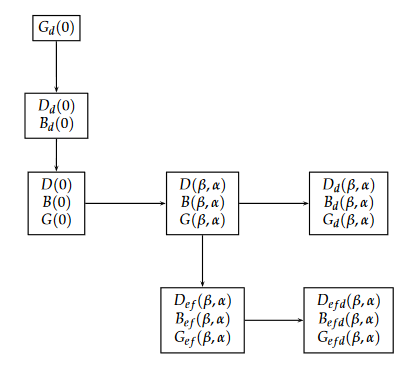
\includegraphics[scale=0.7]{32_ESFBOOK_1}
\centering
\caption{Procedimiendo de cálculo (Figura 3.3 pág 31 \cite{esf_book})}
\label{fig:fig_1}
\end{figure}

En la figura \ref{fig:fig_1} se muestra el proceso de cálculo que se va a seguir para llegar a los valores necesarios para poder estimar la potencia y energía de la instalación.

Los pasos descritos son:
\begin{enumerate}
	\item Separar la irradiación global diaria en el plano horizontal en sus componentes de irradiación difusa y directa.
	\item Convertir la irradiación diaria a un perfil horario de irradiación global, directa y difusa en en plano horizontal.
	\item Pasar del perfil horario en el plano horizontal a un perfil con la inclinación y orientación indicada por el usuario.
	\item Aplicar las pérdidas relacionadas con el ángulo de incidencia y el nivel de suciedad.
	\item Volver a convertir el perfil horario a unos valores diarios de irradiación global, difusa y directa.
\end{enumerate}

\subsection{Separación de la irradiación global diaria en sus componentes}

Como se ha indicado anteriormente, el primer paso del proceso de cálculo es el de separar la irradiación global diaria en en plano horizontal en sus dos componentes, la directa y la difusa.

Al tener solamente un valor de irradiación por cada uno de los meses, utilizaremos el día promedio de cada mes, ya que es posible demostrar que el promedio mensual coincide con el valor diario correspondiente al denominado día promedio.\\

\pagebreak

Estos doce días promedios son:

\begin{table}[ht]
\centering
\begin{tabular}{|l|l|l|l|l|l|l|l|l|l|l|l|l|}
\hline
Mes   & Ene & Feb & Mar & Abr & May & Jun & Jul & Ago & Sep & Oct & Nov & Dic \\ \hline
$d_n$ & 17  & 45  & 74  & 105  & 135  & 161  & 199  & 230  & 261  & 292  & 322 & 347  \\ \hline
\end{tabular}
\label{tab:dias_promedio}
\caption{Dias promedio}
\end{table}
Para el cálculo de la irradiancia solar que finalmente incide en una superficie localizada en la corteza terrestre será útil distinguir tres componentes diferenciados, comúnmente denominados:

\begin{itemize}
\item Radiación Directa, \textit{B}: representa la fracción procedente en linea directa del Sol.
\item Radiación Difusa, \textit{D}: representa toda la radiación procedente de todo el cielo, excepto del sol, y por tanto incluye todos los rayos dispersados por la atmósfera. Es una radiación que depende del estado de la atmósfera, y variará en función de las condiciones climatológicas.
\item Radiación del albedo, \textit{R}: es aquella fracción de la radiación procedente de la reflexión con el suelo. Habitualmente, supone una contribución muy pequeña, que en algunos casos, como el de este proyecto, puede ser despreciada.
\end{itemize}

La suma de las tres componentes constituyen la denominada irradiancia global:
\begin{equation}
G=B+D+R
\end{equation}
\label{equation:eqn_global_radiation}
\subsubsection{Nomeclatura}

Es importante distinguir, dentro de las ecuaciones que modelan el comportamiento de la radiación solar, la forma de indicar cada componente de la irradiancia, el instante o el período en el que se recibe. 

Es recomendable leer estas expresiones en el orden período, forma, tiempo y lugar utilizando el formato de nomenclatura de la siguiente ecuación
\begin{equation}
	Forma_{tiempo, promedio}(lugar)
\end{equation}

Para expresar el lugar de incidencia caben las siguiente posibilidades:
\begin{itemize}
\item (Orientación, Inclinación) : ($\beta , \alpha$)
\item (Horizontal) : (0)
\item (Superficie perpendicular al vector solar): ($n$)
\item (En el plano del generador): ($I$)
\end{itemize}

Por ejemplo, al escribir $B_{h}(0)$ leeremos irradiación directa (forma) horaria(tiempo) en el plano horizontal(lugar), mientras que $G_{d,m}(I)$ se lee media mensual(período) de la irradiación global(forma) diaria (tiempo) en el plano generador (lugar).

















\chapter{Ejemplo práctico de aplicación}
Una vez llevado a cabo el desarrollo teórico de la aplicación y los cálculos necesarios para llegar a los resultados deseados, el siguiente paso será aplicar estos a un emplazamiento concreto, observar los resultados obtenidos y analizarlos para sacar una conclusión.

Éste capítulo también servirá como una guía detallada de uso de la aplicación, explicando la información a introducir en cada paso y como obtenerlos.

La aplicación está disponible a través del enlace \url{http://solarcalc.app} para utilizarse de manera totalmente gratuita.

\section{Obtención de datos del usuario}

El formulario que se le presenta al usuario para que éste introduzca la información de su emplazamiento es el siguiente:
\begin{figure}[ht]
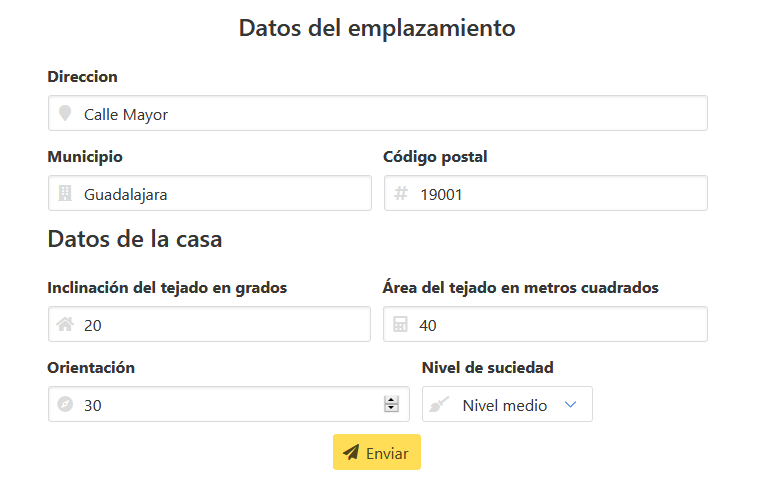
\includegraphics[scale=0.4]{USER_FORM}
\centering
\caption{Formulario web para obtención de datos}
\label{fig:user_form}
\end{figure}

Como se puede observar, el formulario consta de dos partes, por un lado está la dirección como tal, que se utilizará para obtener las coordenadas del emplazamiento y por otro está la configuración física de la superficie destinada a la instalación de los paneles solares.

\subsection{Latitud y longitud a partir de la dirección}

La primera parte del formulario consiste en obtener la información acerca del emplazamiento del usuario, es decir, su latitud y longitud. Estos datos son los que se utilizarán en el código, para obtener la información de la radiación en dicho lugar.

Para ello, el formulario pide una dirección, que no necesariamente tiene que ser la exacta del emplazamiento, sino que se puede utilizar una dirección genérica cercana al lugar donde se va a realizar la instalación, ya que para una distancia relativamente corta la radiación solar no variará de manera notable.

En este caso práctico la dirección que utilizaremos será la de Guadalajara. Para ésta dirección, las coordenadas que Google nos devuelve son:
\begin{itemize}
\item \textbf{Latitud:} $40,632 \degree$.
\item \textbf{Longitud:} $-3.166 \degree$.
\end{itemize}

\subsection{Datos de la superficie destinada a la instalación}

Una vez obtenidas las coordenadas del emplazamiento, es necesario conocer la inclinación, la orientación y el nivel de suciedad de la superficie, para poder realizar el cambio de la radiación en el plano horizontal obtenida anteriormente a la radiación eficaz incidente.

Para ello el formulario nos ofrece 4 campos de información:

\begin{itemize}
\item \textbf{Inclinación en grados:} Para obtener la inclinación de la superficie en grados se puede utilizar cualquier smartphone actual dotado con un sensor giroscópico y una aplicación de tipo nivel, algún dispositivo de medición de ángulos como un transportador.
\item \textbf{Orientación:} Para la obtener la orientación de la superficie se puede utilizar una brújula, ya sea analógica o digital. Se considera que 0 grados es el SUR.
\item \textbf{Área del tejado:} Simplemente el área que se desea cubrir con paneles solares.
\item \textbf{Nivel de suciedad:} Este campo es el mas subjetivo y será a criterio del usuario. Se recomienda realizar cálculos con el peor caso para establecer un margen pero, no obstante, si se conoce con seguridad cuál es el nivel de suciedad de la zona, se ha de usar éste.
\end{itemize}

\section {Aplicación de los datos al proceso de cálculo}

En la sección anterior hemos recogido los datos que un usuario ha introducido a través del formulario. Estos datos son:
\begin{itemize}
\item \textbf{Latitud:} $40,632 \degree$.
\item \textbf{Longitud:} $-3.166 \degree$.
\item \textbf{Inclinación de la superficie:} $20 \degree$.
\item \textbf{Área de la superficie:} $40 m^2 $.
\item \textbf{Orientación de la superficie:} $30 \degree$.
\item \textbf{Nivel de suciedad:} Medio.
\end{itemize}

A continuación, utilizaremos estos datos para recorrer numéricamente el proceso teórico descrito en el capítulo anterior. 

\subsection{Valores medios mensuales de radiación global}

Tal y como se menciona en la sección \ref{section:get_global_rad}, el primer paso para poder llevar a cabo el proceso de cálculo de la radiación incidente eficaz es obtener la radiación global media para cada uno de los doce meses, en el emplazamiento indicado por el usuario.

Para las coordenadas introducidas por el usuario, el punto con información mas cercano que tenemos es de latitud  $40,57 \degree$ y longitud $-3.16 \degree$. 

Para este punto, los valores de irradiación media son:
\begin{table}[ht]
\centering
\begin{tabular}{|l|l|l|l|l|l|l|l|l|l|l|l|l|}
\hline
$kWh/m^2$   & Ene & Feb & Mar & Abr & May & Jun & Jul & Ago & Sept & Oct & Nov & Dic \\ \hline
Valor medio & 2,0 & 3,1 & 4,8 & 5,7 & 6,8 & 8,0 & 7,8 & 6,8 & 5,1  & 3,5 & 2,2 & 1,7 \\ \hline
\end{tabular}
\label{tab:mean_values_monthly}
\caption{Irradiación global media mensual}
\end{table}

\subsection{Irradiancia extra-terrestre diaria}

Además, por otro lado, para poder continuar con el proceso de cálculo, es necesario calcular la irradiancia extra-terrestre diaria, utilizando la latitud indicada por el usuario y los días promedio de la tabla \ref{tab:dias_promedio}.
En las ecuaciones de la sección \ref{section:extra-irrad} se indican los pasos a seguir y el resultado es:
\begin{table}[ht]
\centering
\begin{tabular}{|l|l|l|l|l|l|l|l|l|l|l|l|l|}
\hline
$kW/m^2$   & Ene & Feb & Mar & Abr & May & Jun & Jul & Ago & Sept & Oct & Nov & Dic \\ \hline
$B_{0d}(0)$ & 4,12 & 5,48 & 7,47 & 9,57 & 11,01 & 11,59 & 11,26 & 10,01 & 8,05 & 5,90  & 4,30 & 3,58 \\ \hline
\end{tabular}
\label{tab:extra_irrad_values}
\caption{Irradiancia extra-terrestre diaria}
\end{table}

\subsection{Separación de la radiación global horizontal en sus componentes}

Una vez conocidos los valores mensuales de la radiación global en el plano horizontal, el siguiente paso se centra en separar la radiación global en sus dos componentes, la directa y la difusa, tal y como se explica en la sección \ref{section:radiation_components}.

Como podemos observar en la ecuación \ref{eqn:ktd}, el primer paso para separar la irradiación global en sus dos componentes es calcular el índice de claridad, para que posteriormente calculemos la fracción de radiación difusa. 
\newpage

Si aplicamos dicha ecuación a los resultados anteriores obtenemos los siguiente resultados:

\begin{table}[ht]
\centering
\begin{tabular}{|l|l|l|l|l|l|l|l|l|l|l|l|l|}
\hline
    & Ene & Feb & Mar & Abr & May & Jun & Jul & Ago & Sept & Oct & Nov & Dic \\ \hline
$K_{Td}$ & 0,485 & 0,565 & 0,642 & 0,595 & 0,617 & 0,690 & 0,692 & 0,679 & 0,632 & 0,592 & 0,511  & 0,461  \\ \hline
\end{tabular}
\label{tab:clarity_index}
\caption{Índice de claridad}
\end{table}

A continuación, utilizando la ecuación de Page \ref{eqn:page}, con el índice de claridad calculado, podemos calcular la fracción de difusa:

\begin{table}[ht]
\centering
\begin{tabular}{|l|l|l|l|l|l|l|l|l|l|l|l|l|}
\hline
   		& Ene   & Feb   & Mar   & Abr   & May   & Jun   & Jul   & Ago   & Sept  & Oct   & Nov    & Dic    \\ \hline
$F_{D}$ & 0,452 & 0,361 & 0,274 & 0,327 & 0,302 & 0,220 & 0,218 & 0,232 & 0,285 & 0,330 & 0,421  & 0,478  \\ \hline
\end{tabular}
\label{tab:difuse_part}
\caption{Fracción de difusa}
\end{table}

Con estos valores, utilizando las ecuaciones \ref{eqn:rad_difusa} y \ref{eqn:rad_directa} podemos obtener las dos componentes de la radiación en el plan horizontal.

\begin{table}[ht]
\centering
\begin{tabular}{|l|l|l|l|l|l|l|l|l|l|l|l|l|}
\hline
$kWh/m^2$  & Ene   & Feb   & Mar   & Abr   & May   & Jun   & Jul   & Ago   & Sept  & Oct   & Nov    & Dic    \\ \hline
$B_{d}(0)$ & 1,096 & 1,980 & 3,484 & 3,835 & 4,745 & 6,239 & 6,103 & 5,220 & 3,647 & 2,344 & 1,272  & 0,886  \\ \hline
$D_{d}(0)$ & 0,904 & 1,120 & 1,316 & 1,865 & 2,055 & 1,761 & 1,697 & 1,580 & 1,453 & 1,156 & 0,928  & 0,814  \\ \hline
\end{tabular}
\label{tab:rad_components}
\caption{Irradiación directa y difusa en el plano horizontal}
\end{table}

\subsection{Irradiancia en la superficie inclinada}

\subsubsection{Irradiancia en el plano horizontal}
Conociendo ya los valores diarios de la radiación directa y difusa en el plano horizontal, el próximo paso es obtener los valores horarios de irradiancia, tanto directa como difusa, en el plano horizontal para poder llevar a cabo posteriormente, la traslación de estos valores al plano inclinado.El proceso se describe detalladamente en las secciones \ref{section:3.5.1} y \ref{section:3.5.2}.

Al tratarse de 24 valores horarios, para cada uno de los 12 meses, en total tendríamos 288 valores. Por tanto, y con el fin de no saturar este documento con demasiado valores, se van a indicar los resultados de solamente uno de los meses, en concreto de julio. Estos resultados se muestran en la tabla \ref{tab:hourly_horizontal_values}

\begin{table}[ht]
\centering
\begin{tabular}{|c|r|r|r|r|r|}
\hline
 &
  \multicolumn{1}{c|}{$r_D$} &
  \multicolumn{1}{c|}{$r_G$} &
  \multicolumn{1}{c|}{\begin{tabular}[c]{@{}c@{}}$B_h$\\ ($kW/m^2$)\end{tabular}} &
  \multicolumn{1}{c|}{\begin{tabular}[c]{@{}c@{}}$D_h$\\ ($kW/m^2$)\end{tabular}} &
  \multicolumn{1}{c|}{\begin{tabular}[c]{@{}c@{}}$G_h$\\ ($kW/m^2$)\end{tabular}} \\ \hline
-12 & -0,056 & -0,027 & 0     & 0     & 0     \\ \hline
-11 & -0,053 & -0,026 & 0     & 0     & 0     \\ \hline
-10 & -0,045 & -0,024 & 0     & 0     & 0     \\ \hline
-9  & -0,031 & -0,018 & 0     & 0     & 0     \\ \hline
-8  & -0,014 & -0,009 & 0     & 0     & 0     \\ \hline
-7  & 0,006  & 0,004  & 0,022 & 0,010 & 0,032 \\ \hline
-6  & 0,027  & 0,022  & 0,122 & 0,047 & 0,169 \\ \hline
-5  & 0,049  & 0,042  & 0,248 & 0,083 & 0,331 \\ \hline
-4  & 0,069  & 0,065  & 0,388 & 0,117 & 0,506 \\ \hline
-3  & 0,086  & 0,086  & 0,527 & 0,146 & 0,673 \\ \hline
-2  & 0,099  & 0,104  & 0,645 & 0,169 & 0,814 \\ \hline
-1  & 0,108  & 0,116  & 0,724 & 0,183 & 0,907 \\ \hline
0   & 0,111  & 0,121  & 0,752 & 0,188 & 0,940 \\ \hline
1   & 0,108  & 0,116  & 0,724 & 0,183 & 0,907 \\ \hline
2   & 0,099  & 0,104  & 0,645 & 0,169 & 0,814 \\ \hline
3   & 0,086  & 0,086  & 0,527 & 0,146 & 0,673 \\ \hline
4   & 0,069  & 0,065  & 0,388 & 0,117 & 0,506 \\ \hline
5   & 0,049  & 0,042  & 0,248 & 0,083 & 0,331 \\ \hline
6   & 0,027  & 0,022  & 0,122 & 0,047 & 0,169 \\ \hline
7   & 0,006  & 0,004  & 0,022 & 0,010 & 0,032 \\ \hline
8   & -0,014 & -0,009 & 0     & 0     & 0     \\ \hline
9   & -0,031 & -0,018 & 0     & 0     & 0     \\ \hline
10  & -0,045 & -0,024 & 0     & 0     & 0     \\ \hline
11  & -0,053 & -0,026 & 0     & 0     & 0     \\ \hline
\end{tabular}
\caption{Irradiancia directa, difusa y global en el plano horizontal para el día promedio del mes de julio \label{tab:hourly_horizontal_values}}
\end{table}

\subsubsection{Traslación de los valores al plano horizontal}

Una vez obtenidos los valores horarios en el plano horizontal, podemos trasladar estos al plano inclinado con el proceso descrito de la ecuación \ref{eqn:B_beta_alpha} hasta la ecuación \ref{eqn:ang_incid}. Los resultados se muestran en la tabla \ref{tab:hourly_tilted_values}.

\begin{table}[ht]
\centering
\begin{tabular}{|c|r|r|r|r|r|}
\hline
kW/m^2 &
  \multicolumn{1}{c|}{$B(\beta, \alpha)$} &
  \multicolumn{1}{c|}{$D^C(\beta, \alpha)$} &
  \multicolumn{1}{c|}{$D^I(\beta, \alpha)$} &
  \multicolumn{1}{c|}{$D(\beta, \alpha)$} &
  \multicolumn{1}{c|}{$G(\beta, \alpha)$} \\ \hline
-12 & 0     & 0     & 0     & 0     & 0      \\ \hline
-11 & 0     & 0     & 0     & 0     & 0      \\ \hline
-10 & 0     & 0     & 0     & 0     & 0      \\ \hline
-9  & 0     & 0     & 0     & 0     & 0      \\ \hline
-8  & 0     & 0     & 0     & 0     & 0      \\ \hline
-7  & 0     & 0     & 0,006 & 0,006 & 0,006  \\ \hline
-6  & 0     & 0     & 0,025 & 0,025 & 0,025  \\ \hline
-5  & 0,076 & 0,011 & 0,041 & 0,052 & 0,128  \\ \hline
-4  & 0,243 & 0,037 & 0,052 & 0,089 & 0,3314 \\ \hline
-3  & 0,422 & 0,064 & 0,059 & 0,123 & 0,545  \\ \hline
-2  & 0,583 & 0,088 & 0,064 & 0,152 & 0,735  \\ \hline
-1  & 0,704 & 0,106 & 0,066 & 0,172 & 0,8767 \\ \hline
0   & 0,770 & 0,116 & 0,066 & 0,182 & 0,952  \\ \hline
1   & 0,771 & 0,116 & 0,066 & 0,182 & 0,953  \\ \hline
2   & 0,708 & 0,106 & 0,064 & 0,170 & 0,879  \\ \hline
3   & 0,593 & 0,089 & 0,059 & 0,149 & 0,742  \\ \hline
4   & 0,443 & 0,067 & 0,052 & 0,119 & 0,562  \\ \hline
5   & 0,277 & 0,042 & 0,041 & 0,082 & 0,349  \\ \hline
6   & 0,119 & 0,018 & 0,025 & 0,043 & 0,162  \\ \hline
7   & 0,010 & 0,001 & 0,006 & 0,007 & 0,017  \\ \hline
8   & 0     & 0     & 0     & 0     & 0      \\ \hline
9   & 0     & 0     & 0     & 0     & 0      \\ \hline
10  & 0     & 0     & 0     & 0     & 0      \\ \hline
11  & 0     & 0     & 0     & 0     & 0      \\ \hline
\end{tabular}
\caption{Irradiancia directa, difusa y global en el plano inclinado, para el día promedio del mes de julio \label{tab:hourly_tilted_values}}
\end{table}
\newpage

Como se  puede observar, a diferencia de la irradiancia en el plano horizontal, estos resultados no son simétricos respecto al mediodía ya que ahora está afectando la orientación de la superficie, que no está orientada totalmente hacia el sur.

\chapter{Conclusión}

\appendix
\chapter{Anexo I: Detalles de la programación}


\pagebreak

\begin{thebibliography}{99}

\bibitem{unef_2019} Unión Española Fotovoltaica. 2019. Informe anual 2019: El sector fotovoltaico impulsor de la transición energética. \url{https://unef.es/wp-content/uploads/dlm_uploads/2019/09/memoria_unef_2019-web.pdf}.  
\bibitem{sota_pvsyst} PVSyst. PVsyst SA.  \url{https://www.pvsyst.com/download-pvsyst/}.  
\bibitem{sota_calculationsolar} CalculationSolar. 2014. \url{http://www.calculationsolar.com/}.
\bibitem{sota_sisifo} SISIFO.Instituto de Energía Solar.  \url{https://www.sisifo.info/es/default}.  
\bibitem{sota_pvgis} PVGIS. European Commission, Joint Research Centre. \url{https://re.jrc.ec.europa.eu/pvg_tools/es/tools.html}.  
\bibitem{sota_sam} System Advisor Model. NREL, US Department of Energy \url{https://sam.nrel.gov/}.
\bibitem{sota_solaR}   Oscar Perpiñán (2012). solaR: Solar Radiation and Photovoltaic
  Systems with R, Journal of Statistical Software, 50(9), 1-32. \url{http://www.jstatsoft.org/v50/i09/}.  
\bibitem{esf_book} Perpiñán, O. 2018. Energía Solar Fotovoltaica. \url{http://oscarperpinan.github.io/esf/}.

\bibitem{lj60}B. Y. H. Liu y R. C. Jordan. “The interrelationship and characteristic distribution of direct,diffuse, and total solar radiation”. \textit{Solar Energy} 4 (1960), págs. 1-19
\bibitem{temp_paper} Estimating average daytime and daily temperature profiles within Europe.  Thomas A.Huldm Marcel Šúri, Ewan D.Dunlop, Fabio Micale 2006  \url{https://www.sciencedirect.com/science/article/abs/pii/S1364815205001593}

\end{thebibliography}


\end{document}
